
   %%%%%%%%%%%%%%%%%%%%%%%
 %%%  NOAH'S SUPER COOL  %%%
%%%%      ACADEMIC       %%%%
 %%%   LATEX TEMPLATE    %%%
   %%%%%%%%%%%%%%%%%%%%%%%

\documentclass[12pt]{article}
\usepackage[letterpaper]{geometry}
\geometry{top=1in, bottom=1in, left=1in, right=1in}
\usepackage{fontspec}
\usepackage{tgtermes}
\usepackage{hanging}
\setmainfont[
 ItalicFont={texgyretermes-italic.otf},
 BoldFont={texgyretermes-bold.otf},
 ]{texgyretermes-regular.otf}
\usepackage{setspace}
\doublespacing
\usepackage{graphicx}
\graphicspath{ {./graphics/} }

\begin{document}

% Title Page
\pagenumbering{gobble} % remove page numbers
\begin{center}
\topskip0pt
\vspace*{\fill}
Air Resistance Lab 7 \\ Noah Dinan \\ PHY 1110 - Mayer \\ \today \\
\vspace*{\fill}
\end{center}

\newpage
\pagenumbering{arabic} % resume page numbering

\setlength{\parindent}{0in}

\textbf{Results}

For this lab report, a paper cone was dropped from a height of 2 meters.
Because of the light weight of the cone, the drag force of air resistance is not negligible.

Our primary source of systematic error was innacuracies while timing the cone falling.
We attempted to lessen this error bu averaging three values to find the time for each trial.

Below is the equation for calculating drag force.

\[ma = mg - F_{drag} \]

Because velocity is constant, $ ma = 0 $ as the cone is not accelerating. Therefore $ mg = F_{drag} $.

Once we found the values for $ F_{drag} $, we graphed $ F_{drag} $ with respect to $v$ and $v^2$, resulting in the following
graphs.

\newpage

\begin{center}
    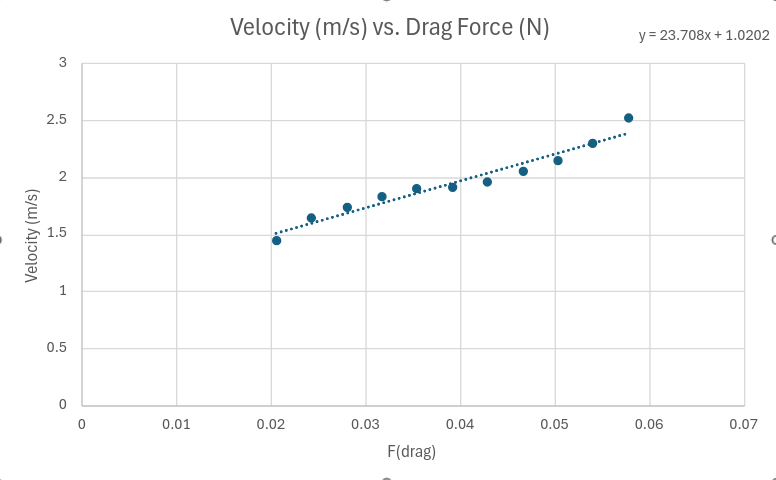
\includegraphics[scale=0.60]{v_vs_drag.png}
    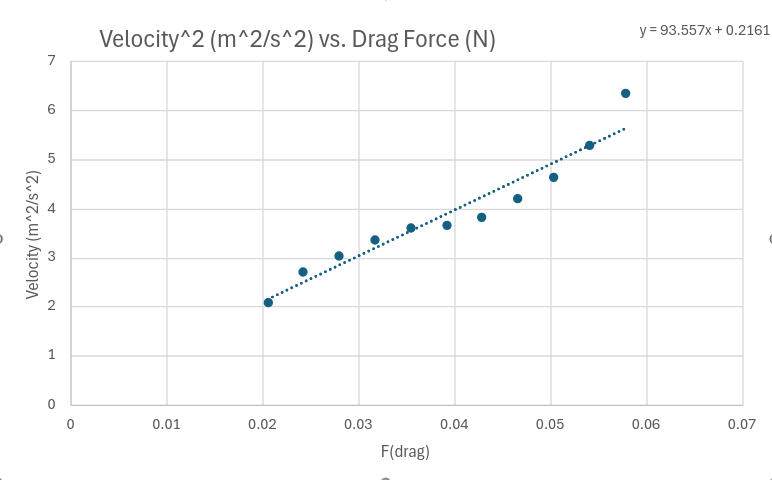
\includegraphics[scale=0.60]{v2_vs_drag2.png}
\end{center}

The theory of air resistance states that there are two forms of air flow, generally dependent on the shape of the object falling:
Laminar airflow is smooth and has a $n$ value closer to 1, whereas turbulent air flow gives an $n$ value closer to 2.

The equation below shows the relationship between $F_{drag}$ and velocity.

\[ F_{drag}(v) = k_3v^n \]

To find a value for $n$ and $k_3$, we graphed $\ln(F_{drag}) vs \ln(v)$ (shown below) and find the y-intercept and slope.

\begin{center}
    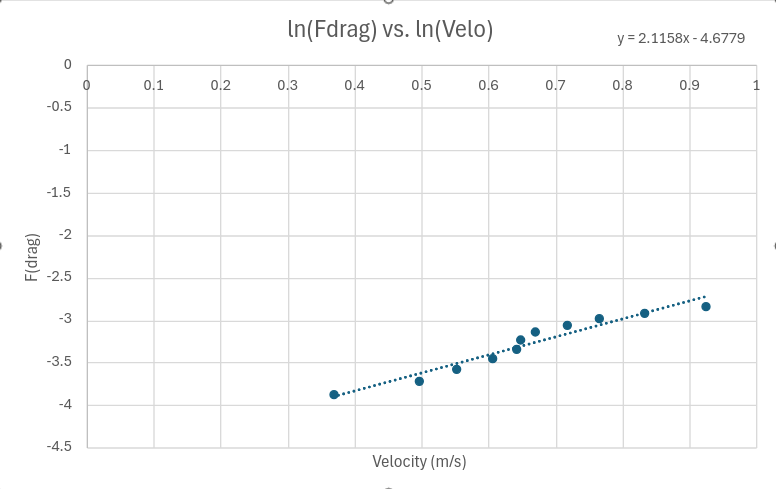
\includegraphics[scale=0.60]{lnv_lndrag.png}
\end{center}

\textbf{Conclusions}

Using this graph, we found $n = 2.1158$ and $k_3 = e^{-4.6779} = 0.009298$.
The value for $n$ being greater than 2 shows that we likely had some systematic error but overall airflow is turbulent, not Laminar.
The value for $n$ is not equal to 1 so the drag force is not proportional to velocity for the experiment.
Our value for $k_3$ is likely so small because we converted our values to SI units early on in the experiment to ensure
consistency.


\end{document}
